\chapter{Theoretical part}

\section{History of virtualization}

\paragraph{While computer technology continues to march forward with smaller, sleeker, more powerful machines, in many ways how we use computers has come full circle.
Obviously the computers of today are way more powerful than the computers of the 1950s, but it turns out the way we are using them is going back to the early days 
of computing.}

\paragraph{Anyone who has been around computers for a while will quickly recognize that the concept of running a client’s session on a server and then displaying the 
results on the client machine describes the way mainframes work.  Let’s take a look at the history of virtualization to see how it all began and look at some of the 
ways that the world of virtualization has evolved.}

\section{Mainframes examples}

\textbf{VMware}
\paragraph{The reigning king in the world of virtualization is VMware. Their line of products (including ESX Server and VI3) has led the recent movement toward 
virtualized IT systems.}

\textbf{Connectix Corp}
\paragraph{Connectix Corp. was a company that made virtualization software for Windows and Macintosh-based computers. In 2003 Microsoft acquired their virtualization 
technology and now uses it in their own virtualization products.}

\textbf{Microsoft}
\paragraph{In addition to Hyper-V (the main subject of this book ), there are two other virtualization products from Microsoft out there. 
While not as grand in scope as Hyper-V, they are still a means of virtualization. Microsoft brings to the virtualization party Virtual PC, Virtual Server, and Hyper-V. }


\section{What is Hyper-V}

\paragraph{Following the launch of Windows Server 2008, Microsoft released Windows Server 2008 Hyper-V, the hypervisor-based virtualization technology that is a role 
built into 64-bit versions of Windows Server 2008. Hyper-V offers a reliable, scalable, and high-performance virtualization platform that plugs into existing IT 
infrastructures, enabling users to consolidate some of the most demanding workloads. In addition, the Microsoft System Center product family gives customers a single 
set of integrated tools to manage physical and virtual resources, helping customers create a more agile and dynamic datacenter. Hyper-V’s scalability derives from its 
support for multiple processors and cores at the host level and improved memory limits at the host and guest level within virtual machines. This enables users to scale 
their virtualization environment to support a large number of virtual machines within a given host and to take advantage of quick migration for high availability across 
multiple hosts.}

\section{What is a v-switch}

\paragraph{A \textbf{v-switch}, ( virtual switch more precise ), is a virtual device that give the virtual machines and the host to communicate over network.
This type of switches are completely simulating a real swithc, giving a network admin the posibility to create complex routes and networks, faster and easier that working
with physical devices. In most cases, a v-switch is used to create communication channels vetween Virtual Machines, and between virtual machines and the host.}

\subsection{Networking options}

By default Hyper-V comes with three different networking settings: 
\begin{enumerate}
\item \textbf{External}
\item \textbf{Internal}
\item \textbf{Private} 
\end{enumerate}

\paragraph{The \textbf{External} network setting creates a connection to a physical NIC so that guest virtual machines can access the physical network to which that NIC is connected. 
The \textbf{Internal} setting creates a network that the host and the guest virtual machines can communicate on. The \textbf{Private} network setting creates a network that only virtual 
machines can communicate on. The main and only difference betweem Internal and Private is that the host machine does not have a NIC in the Private one. Basicly, if you add a NIC of the 
host in a Private network, it becomes an Internal one. More than likely, if you are mixing production, development, and test workloads on your virtual environments, you will have a mix 
of external, internal, and private networks.}

\subsection{What can be filtered}

\paragraph{A normal firewall, working on a machine, can have access to traffic data at the 7th from the OSI model, and more exactly at the Application Layer.
When talking about filtering traffic from a switch, the maximum layer that we can access is layer 4, and more exactly the Transport Layer.}

\paragraph{The difference between the 2 aproaches is that filtring at layer 7 gives you more control over what applications access the network, or what applications
are accessed from outside the computer. Layer 7 gives us information like \textbf{Application id} and \textbf{TCP Flow Information}}.

\begin{figure}[h]
\centering
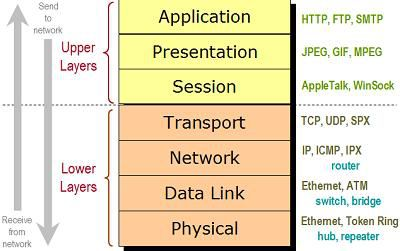
\includegraphics[width=1\textwidth]{osi-stack.jpg}
\caption{OSI Stack}
\label{osi-stack}
\end{figure}

\subsubsection{TCP example}

\paragraph{TCP has a well known \textit{handshake} for every connection made. It is a way to syncronize 2 endpoints and let them know how to communicate with each other.
The handshake looks like this:}
\begin{enumerate}
\item A pachet that has \textbf{SYN} TCP flag set, is sent from the client to server.
\item A pachet that has \textbf{SYN-ACK} TCP flags set, is sent from the server to client.
\item A pachet that has \textbf{ACK} TCP flag set, is sent from the client to server.
\end{enumerate}
\paragraph{After this operation, at the operating system level, the TCP connection has been made. This connection is known as a \textbf{TCP Flow}. On a Windows machine,
the NDIS network drivers does this, with the help of tcpip.sys driver.}
\paragraph{It is important to notice the fact that when working on Layer 7 as a firewall, you can detect and make a decision about every TCP Flow, without bothering with
the handshake. On the other hand, if a firewall wants to filter traffic from the siwtch, it must correlate by itself all the handhake operations to detect a TCP connection.}

\subsubsection{Traffic directions}
\paragraph{At the machine layer, when talking about network traffic we have inbound traffic, and outbound traffic. As their name sais, inbound traffic is the one that comes from
outside and outbound traffic is the one that goes out in the network. When speaking about v-swith traffic, there is no inbound and outbound, because the refference object os not 
a machine anymore, but a switch. For these, there are the terms \textbf{Egress} and \textbf{Ingress}. \textbf{Egress} traffic is the traffic that gets out from the switch,
and \textbf{Ingress} is the traffic that goes in the switch. }


\begin{figure}[h]
\centering
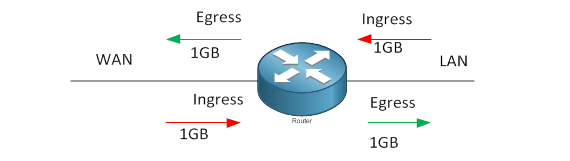
\includegraphics[width=1\textwidth]{ingress-vs-egress.png}
\caption{Ingress vs Egress direction}
\label{ingress-vs-egress}
\end{figure}

\section{Virtualization types}
\section{Hyper-V Partitions}
\subsection{VMBus}
\section{Windows Kernel}
\subsection{File system drivers}
\subsection{Network Drivers(NDIS)}
\section{Network drivers}
\subsection{TCP/IP stack}
\subsection{Windows Filtering Platform}
\subsubsection{Layer available for filtering}
\subsubsection{Filters}
\subsubsection{Callouts}

